\documentclass[
12pt, paper=a4,  listof=totocnumbered, % lists are also included in table of contents
, % Don't add a period at the end of a chapter number
]{scrreprt}

\usepackage{chngcntr}
    \counterwithout{footnote}{chapter}
    \counterwithout{figure}{chapter}

% get custom bibliography style working without prepending [brackets]
\usepackage{natbib}

%\setcitestyle{aysep={}} % remove comma as delimiter 

% breaks line at hyphens (resolves formatting issues in bibliography)
\usepackage[hyphens]{url}


% if you insist on Arial... then uncomment the following
\usepackage{helvet}
\renewcommand{\familydefault}{\sfdefault}

\usepackage[left=2.5cm,right=2.5cm,top=2.5cm,bottom=2.5cm]{geometry} % margins
%\addtolength{\footskip}{-0.7cm}% foot larger by 0,7 cm  (Raises the page number)


%\usepackage[onehalfspacing]{setspace} % line space 1,5
\usepackage[doublespacing]{setspace}
%\doublespacing

%\setlength{\parindent}{12pt} % Indent at start of paragraphs  6pt

\usepackage[utf8]{inputenc} %UTF-8 to encode many characters => for many characters, you can just input the character and avoid a macro

\usepackage[english]{babel} % english hyphenations
%\usepackage[T1]{fontenc} %wichtig für Trennung von Wörtern mit Umlauten
\usepackage{microtype} % align margins


\usepackage{graphicx} % import graphics
\usepackage{placeins}% places the graphics within text

% Abbreviation's directory
% printonlyused - only if used
% withpage - the first occurrence's page number is listed too
\usepackage[withpage]{acronym}

% for tables
\usepackage{longtable}
\usepackage{multirow}

\usepackage[hidelinks]{hyperref} %https://tex.stackexchange.com/questions/823/remove-ugly-borders-around-clickable-cross-references-and-hyperlinks


\begin{document}

%\renewcommand{\thechapter}{\Roman{chapter}}
%TITELBLATT:!!!!!!!!!!!!!!!!!!!!!!!!!!!!!!!!!!!!!!!!!!!!!!!!!!!!!!!!!!!!!!!!!!!!!!!!!!!!!!!!!!!!!!!!!!!!!

\label{titlePage}
\begin{figure}[h]
\centering

\includegraphics[width=0.50\textwidth]{pics/logo.pdf}
\end{figure}
\FloatBarrier

\begin{Large} 
\begin{center}
Launching into Cybersecurity
\end{center}
\end{Large} 

\vspace*{5mm}

\begin{large} 
\begin{center}
University of Essex
\end{center}
\end{large} 

\begin{large} 
\begin{center}
Study-branch: MSc. Cyber Security
\end{center}
\end{large}



\begin{Large} 
\begin{center}
\textbf{Final Report}
\end{center}
\end{Large}

\vspace*{5mm}


\begin{large} 
\begin{center}
Advisor: Dr. Sabeen Tahir
\end{center}
\end{large} 


\vspace*{-6mm}

\begin{large} 
\begin{center}
Delivery date: 21.11.2022
\end{center}
\end{large} 


\pagestyle{empty} % no page numbering on the cover



\renewcommand{\thechapter}{\Roman{chapter}}

\pagestyle{plain}

\pagenumbering{Roman} %the intro is counted with roman numbers
\setcounter{page}{2} %starting with page 2 (page 1 is the titel)

\tableofcontents %table of contents
\listoffigures %List of figures
\listoftables %list of tables

% Abbreviations list
\renewcommand\refname{Abbreviations} \chapter{Abbreviations}
% The abbreviations list should contain all abbreviations that are not common-knowledge.
\begin{acronym}[NMWC] % the longest abbreviation here (for layout)
    \setlength {\itemsep}{-\parsep} % geringerer Zeilenabstand    	 

    \acro{ASMIS}{Appointment Scheduling Management Information System}
    \acro{MFA} {Multi factor Authentication}
    \acro{OWASP} {Open Web Application Security Project®}
    \acro{SSDLC}{Secure Software Development Lifecycle}
    \acro{UML}{Unified Modeling Language}
    

\end{acronym}

% Acronyms should be made hyperreffed the first time they appear in text with
% \ac{CI}  

\renewcommand{\thechapter}{\arabic{chapter}} %Count chapters with arabic numbers and not roman numbers
\setcounter{chapter}{0} %Reset chapter counter
\pagenumbering{arabic}

\chapter{Introduction}
The healthcare sector is a vital part of our lives, and went through countless advancements in this field, improving our livelihood. The mere thought of not having accessible healthcare is catastrophic and can lead to countless loss of lives. Therefore, we must take great caution in improving communication between patients and healthcare providers to ensure everyone gets the proper required service.\newline \newline
Similarly, Queens Medical Center is one of many healthcare centers serving the 
residents as the first point of contact for any health-related issues. The new automated appointment system will provide a web interface between the clinic and the patient, where patients can easily book an appointment using a computer or a mobile device with access to the internet.\newline\newline
Deployment of the ASMIS system has numerous benefits, namely, saving human resources and time. The medical staff is already under large workloads, and with this system, they can redirect their energy to other sectors. The system also has positive effects on the user's side, where patients do not have to wait for clinic personnel to pick up the phone; instead, they open the application and book an appointment instantly. In particular, automation drastically reduces human error in scheduling, which could sometimes be a matter of life and death. In the long run, digitalization will save more money and make the system more efficient.\newline\newline
Using the ASMIS system has its advantages but, is not free from the vulnerabilities that cyberspace brings along. For the application to work as intended, it needs to store the personal data of the patient, specialists, and other staff. Storing such Personally Identifiable Information (PII) creates a significant risk to privacy \citep[p.~374]{IOT}. If data is stolen or leaked, crooks can use the data for illegal activities or sell it. In addition to data leaks, the danger is always lurking, which could disrupt the functionality of critical infrastructure. External threats, such as DDoS attacks, malware, viruses, and advanced persistent threats, are more everpresent. These attacks cause financial, reputational damage, and damage to lives \citep[p.~377]{IOT}.\newline\newline
The main aim of this report is to analyze different threats and levels of risks present in the system. Threat modeling and risk managing techniques will lead to a more robust and secure Appointment Scheduling Management Information System (ASMIS) and raise user confidence.
\chapter{ASMIS Use Cases}

\begin{figure}[h!]
\centering
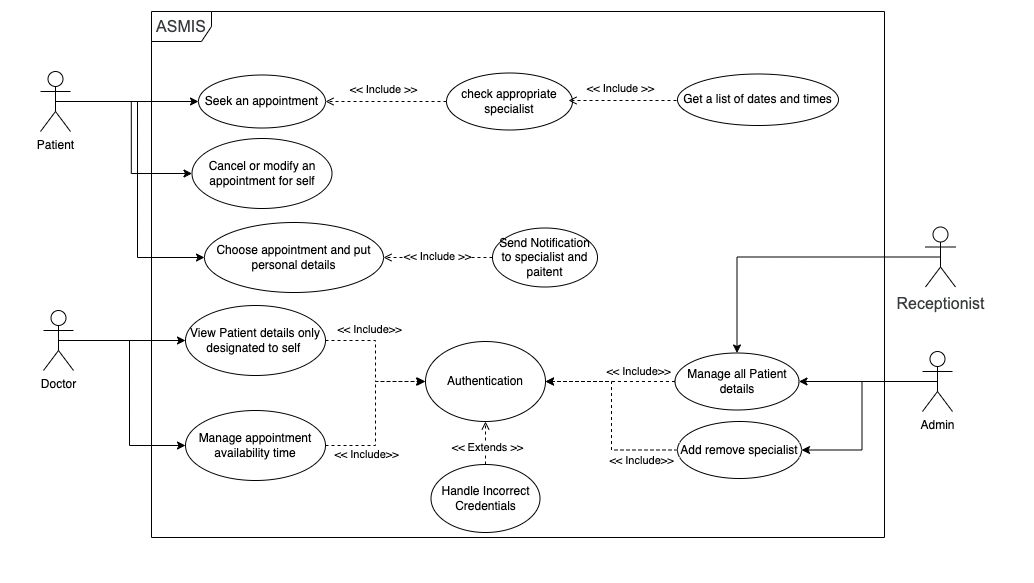
\includegraphics[width=\textwidth]{pics/usecase.png}
\caption{Use case diagram for ASMIS}\label{fig:usecase}
\end{figure}

\section{Overview}
The use case is a very insightful UML diagram that allows us to capture, identify, and analyze the system under development. The diagram analyzes the system by dividing the actions possible using different actors \citep[p.~64]{jacobson2021unified}. In this case, the use case shows us the possible paths to be available for the ASMIS application and could be the base to apply an abuse case threat modeling \citep [p.~59]{usecase_abuse_case}.


\section{Analyzing Use Case}
Figure \ref{fig:usecase} depicts a use case diagram for the ASMIS system for the Queens medical center. This application will provide a platform for the patient and the clinic staff to manage and operate the scheduling efficiently and swiftly. \newline\newline
The application consists of four main actors the patient, the doctor/specialist, the receptionist, and the admin. The patient can seek an appointment using the application without logging in by inputting the desired health-related issue. After this step, the application determines the appropriate specialists for the patient and presents the list of available appointments. Lastly, the patient chooses the date and the specialist with personal data, including name, address, email, and phone number, which would send a confirmation email.\newline\newline
From the use case diagram, one can see that specialists and admin can manage the appointment schedules and also check the patient who booked an appointment. The main difference between the admin, the receptionist, and the specialist is the right to see data. The specialist can only see the patient data assigned to own, but admins and receptionists can manage all patient data. Similarly, the other actors, the specialist, the receptionist, and the admin, must authenticate to carry out any actions. Additionally, the admins can add and remove specialists and receptionists in the system and allocate them privileges. 
\chapter{Threat Modeling}
Threat modeling is gaining more importance in application development, also known as the Secure Software Development Lifecycle (SSDLC) \citep{snyk_2022}. In the development cycle, one can use threat modeling approaches to identify and analyze different security issues in the application. Many other processes exist to carry out threat modeling, each of which has advantages and disadvantages. However, in this report, the Abuse Case Modelling and the STRIDE method will be used to analyze and recommend appropriate mitigations for the dangers using the recommended process from OWASP \citep{owasp_threat_model_process}.

\section{Threat Model Information}
\textbf{Application Name}: Appointment and Scheduling Management Information System
\textbf{Application Version}: 1.0 \newline
\textbf{Description}: Queens medical center is a community clinic that needs to replace its call-based appointment system with an online web application. Following the use cases (see. figure \ref{fig:usecase}), the application will have four actors/users.
\begin{itemize}
  \item Patients
  \item Receptionist
  \item Specialists/Doctors
  \item Admins
\end{itemize}

\newpage

\section{Trust Levels}
The trust levels define the privileges and grants an external entity/actors receive to use the application. The trust levels defined for the ASMIS system for the Queens medical center are defined in Table \ref{table:trust_levels}

\begingroup
\begin{table}[h!]
\centering
\setlength{\tabcolsep}{6.5pt} % Default value: 6pt
\renewcommand{\arraystretch}{1.8} % Default value: 1
\begin{tabular}{ |p{1cm}|p{6cm}|p{8cm}|}
 \hline
 \textbf{ID} & \textbf{Name} & \textbf{Description} \\ [0.5ex] 
 \hline
 1 & Anonymous Web User/Patient & A user who can schedule an appointment with a specialist without providing valid credentials. However, Personal Identifiable Information is provided during scheduling. \\
 \hline
 2 & Specialist with Valid Login Credentials & A special user who is a doctor/specialist in the clinic. When logged in using valid credentials, he/she can manage, create, modify, and view scheduling information connected to their profile. \\
 \hline
 3 & Receptionist with Valid Login Credentials & A special user who is a receptionist in the clinic. When logged in using valid credentials, he/she can manage, create, modify, and view the scheduling information of all patients. \\
 \hline
 4 & Admin with Valid Login Credentials & A special user who is an Admin in the clinic. When logged in using valid credentials, he/she can manage, create, modify, and view scheduling information connected to all specialist profiles. Additionally, the admin can add new specialists and assign permissions.\\
 \hline
 5 & Database Read/Write User & A database account is used to read and write the contents of the database.  \\ [1ex]
 \hline
\end{tabular}
\caption{Trust Levels ASMIS system.}
\label{table:trust_levels}
\end{table}
\endgroup

\section{Entry Points}
The entry points are the available access points through which users and potential hackers interact with the application. The definition of access points in the threat model aids us in determining from which points the attack vectors are carried out to hinder the application's functionality.\newline

\begingroup
\centering
\setlength{\tabcolsep}{6.5pt} % Default value: 6pt
\renewcommand{\arraystretch}{1.8} % Default value: 1
\begin{longtable}{ |p{3cm}|p{3cm}|p{5cm}| p{3cm} |}
 \hline
 \textbf{ID} & \textbf{Name} & \textbf{Description} & \textbf{Trust Levels} \\ [0.5ex] 
 \hline
 \multirow{2}{5em}{1} & Appointment Scheduling Main Page & The main page for all users of the application & (1) Anonymous Web User \\
 \hline
 \multirow{2}{5em}{2} & Appointment Scheduling Patient Page & The first point of contact for the patient to seek an appointment for their health issues. & (1) Anonymous Web User \\
 \hline
 3 & Login Page & The specialists, receptionists, and admins must log in before carrying out their respective functions & 
 (1)Specialist with Valid Login Credentials \newline
 (2)Receptionist with Valid Login Credentials \newline
 (3)Admin with Valid Login Credentials \newline
 (4)Database Read/Write User
 \\
 \hline
 4 & Appointment Management Page & The page can manage and modify all the information for appointments for a specific specialist & 
 (1)Specialist with Valid Login Credentials \newline
 (2)Receptionist with Valid Login Credentials \newline
 (3)Admin with Valid Login Credentials \newline
 (4)Database Read/Write User\\
 \hline
  5 & Search All Patient Pages & The page can manage and view all the information for patients who scheduled an appointment. & 
 (1)Specialist with Valid Login Credentials \newline
 (2)Receptionist with Valid Login Credentials \newline
 (3)Admin with Valid Login Credentials \newline
 (4)Database Read/Write User
 \\
 \hline
 6 & Admin Page & The page used by the admins to add new users and assign them with needed permissions & 
 (1)Admins with Valid Login Credentials \newline \\
 \hline
 \caption{Entry Points ASMIS system.}
    \label{table:entry_points}
\end{longtable}
\endgroup

\section{Abuse Case Model}

\begin{figure}[h!]
\centering
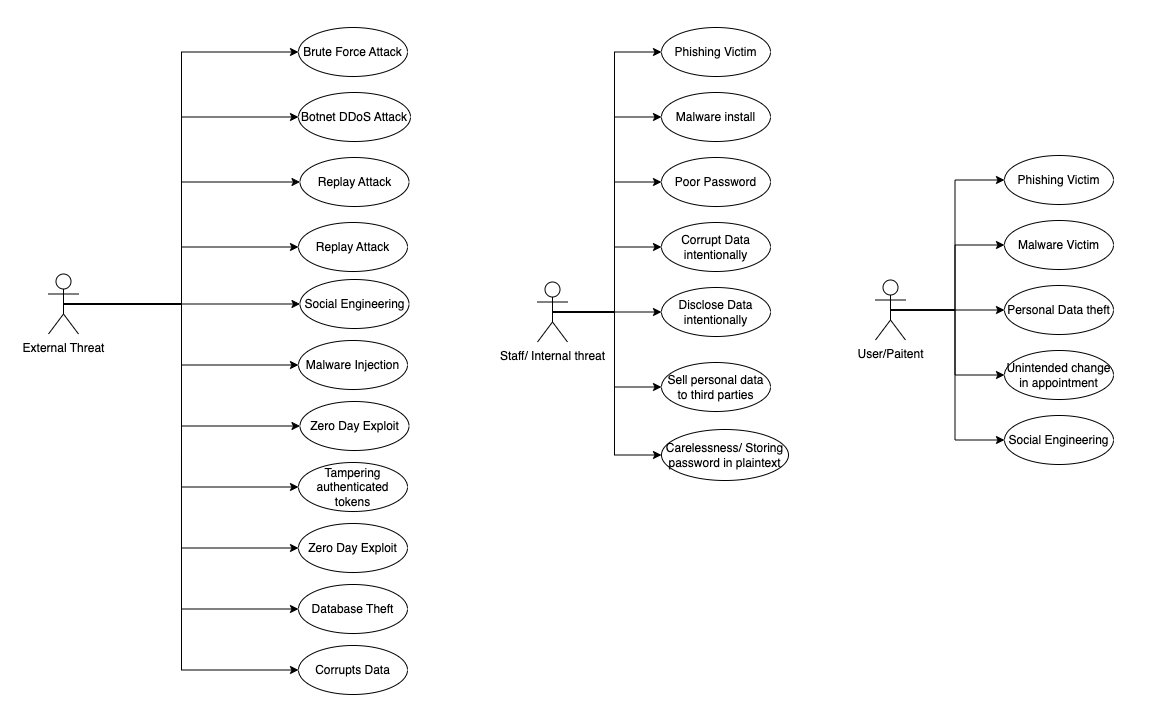
\includegraphics[width=\textwidth]{pics/abusecase.png}
\caption{Abuse case diagram for ASMIS}\label{fig:abuse_case}
\end{figure}

Using the Entry points (See Table \ref{table:entry_points}) and the use cases (See Figure\ref{fig:usecase}) the following possible abuse/misuse cases have been derived.
The possible dangers and the reliability of the ASMIS system are divided into three distinct actors: the external attacker, the staff/internal threat, and the patient/user. Table \ref{table:abuse_case} elaborates the risk factors with the recommended mitigation for the given abuse cases.

\begingroup
\centering
\setlength{\tabcolsep}{6.5pt} % Default value: 6pt
\renewcommand{\arraystretch}{1.8} % Default value: 1
\begin{longtable}{ |p{3cm}|p{3cm}|p{3cm}| p{5cm} |}
 \hline
 \textbf{Threat} & \textbf{Likelihood} & \textbf{Impact} & \textbf{Mitigations} \\ [0.5ex] 
 \hline
 Brute Force Attack & High & Moderate & (1) Block User for a while after X failed log in attempts\newline
 (2) Use fraud detection \newline
 (3) Use strong passwords
 \citep[p.~682-683]{herley2008protecting}\\
 \hline
 DDoS Attack & High & High & (1) Traffic flow Monitoring\newline
 (2) Anomaly Detection using ML \newline
 (3) Define strong and quick remedies in case of an attack
 \citep[p.~1]{DDOS}\\
\hline
   Malware & Moderate & High & (1) Install up-to-date antivirus.\newline
  (2) Use of threat monitoring tools, i.e., Security information and event management (SIEM) tools.\newline
  (3) Recurring Training - how to avoid malware  
  \\
 \hline
 Social Engineering & High & Moderate & (1) Security training and awareness for all users\newline
 (2) Incident Response \citep[p.~ 13-17]{chantler2008social}
  \\
  \hline
   Database Theft & Moderate & High & (1) Encrypt database at rest\newline
 (2) Database User credentials must be stored in a safe place
  \\
  \hline 
     Data corruption by staff & Low & High & (1) Work with least privileges\newline
 (2) Backup data in secure and isolated storage.
  \\
  \hline
       Poor password & High & High & (1) Strong password requirements\newline
       (2) Use MFA in complement with a password.
  \\
  \hline
 \caption{Abuse Case Risk and Mitigation Analysis}
    \label{table:abuse_case}
\end{longtable}
\endgroup





\appendix 

% ---- Bibliography ----
%
% BibTeX users should specify bibliography style 
% References will then be sorted and formatted in the correct style.
%
 %\bibliographystyle{alpha}
\renewcommand{\bibname}{References}
\bibliographystyle{agsm}
\bibliography{biblio}

\end{document}
